%%
%% This is file `sample-manuscript.tex',
%% generated with the docstrip utility.
%%
%% The original source files were:
%%
%% samples.dtx  (with options: `manuscript')
%% 
%% IMPORTANT NOTICE:
%% 
%% For the copyright see the source file.
%% 
%% Any modified versions of this file must be renamed
%% with new filenames distinct from sample-manuscript.tex.
%% 
%% For distribution of the original source see the terms
%% for copying and modification in the file samples.dtx.
%% 
%% This generated file may be distributed as long as the
%% original source files, as listed above, are part of the
%% same distribution. (The sources need not necessarily be
%% in the same archive or directory.)
%%
%% The first command in your LaTeX source must be the \documentclass command.
%%%% Small single column format, used for CIE, CSUR, DTRAP, JACM, JDIQ, JEA, JERIC, JETC, PACMCGIT, TAAS, TACCESS, TACO, TALG, TALLIP (formerly TALIP), TCPS, TDSCI, TEAC, TECS, TELO, THRI, TIIS, TIOT, TISSEC, TIST, TKDD, TMIS, TOCE, TOCHI, TOCL, TOCS, TOCT, TODAES, TODS, TOIS, TOIT, TOMACS, TOMM (formerly TOMCCAP), TOMPECS, TOMS, TOPC, TOPLAS, TOPS, TOS, TOSEM, TOSN, TQC, TRETS, TSAS, TSC, TSLP, TWEB.
% \documentclass[acmsmall]{acmart}
\documentclass[sigconf]{acmart}

%% 追加
\usepackage{bm}
\newcommand\figref[1]{\textbf{Figure~\ref{fig:#1}}}
\newcommand\tabref[1]{\textbf{Table~\ref{tab:#1}}}
\usepackage{url}
\usepackage{color}
\usepackage{multirow}
\usepackage{diagbox}
%% ここまで

%%%% Large single column format, used for IMWUT, JOCCH, PACMPL, POMACS, TAP, PACMHCI
% \documentclass[acmlarge,screen]{acmart}

%%%% Large double column format, used for TOG
% \documentclass[acmtog, authorversion]{acmart}

%%%% Generic manuscript mode, required for submission
%%%% and peer review
% \documentclass[manuscript,screen,review]{acmart}
%% Fonts used in the template cannot be substituted; margin 
%% adjustments are not allowed.
%%
%% \BibTeX command to typeset BibTeX logo in the docs
\AtBeginDocument{%
  \providecommand\BibTeX{{%
    \normalfont B\kern-0.5em{\scshape i\kern-0.25em b}\kern-0.8em\TeX}}}

%% Rights management information.  This information is sent to you
%% when you complete the rights form.  These commands have SAMPLE
%% values in them; it is your responsibility as an author to replace
%% the commands and values with those provided to you when you
%% complete the rights form.
% \setcopyright{acmcopyright}
% \copyrightyear{2018}
% \acmYear{2018}
% \acmDOI{10.1145/1122445.1122456}

% %% These commands are for a PROCEEDINGS abstract or paper.
% \acmConference[Woodstock '18]{Woodstock '18: ACM Symposium on Neural
%   Gaze Detection}{June 03--05, 2018}{Woodstock, NY}
% \acmBooktitle{Woodstock '18: ACM Symposium on Neural Gaze Detection,
%   June 03--05, 2018, Woodstock, NY}
% \acmPrice{15.00}
% \acmISBN{978-1-4503-XXXX-X/18/06}
\copyrightyear{2021}
\acmYear{2021}
\setcopyright{acmcopyright}\acmConference[ISWC '21]{2021 International Symposium
on Wearable Computers}{September 21--26, 2021}{Virtual, USA}
\acmBooktitle{2021 International Symposium on Wearable Computers (ISWC '21),
September 21--26, 2021, Virtual, USA}
\acmPrice{15.00}
\acmDOI{10.1145/3460421.3478823}
\acmISBN{978-1-4503-8462-9/21/09}


%%
%% Submission ID.
%% Use this when submitting an article to a sponsored event. You'll
%% receive a unique submission ID from the organizers
%% of the event, and this ID should be used as the parameter to this command.
%%\acmSubmissionID{123-A56-BU3}

%%
%% The majority of ACM publications use numbered citations and
%% references.  The command \citestyle{authoryear} switches to the
%% "author year" style.
%%
%% If you are preparing content for an event
%% sponsored by ACM SIGGRAPH, you must use the "author year" style of
%% citations and references.
%% Uncommenting
%% the next command will enable that style.
%%\citestyle{acmauthoryear}

%%
%% end of the preamble, start of the body of the document source.
\begin{document}

%%
%% The "title" command has an optional parameter,
%% allowing the author to define a "short title" to be used in page headers.
\title{disp2ppg: Pulse Wave Generation to PPG Sensor using Display}

%%
%% The "author" command and its associated commands are used to define
%% the authors and their affiliations.
%% Of note is the shared affiliation of the first two authors, and the
%% "authornote" and "authornotemark" commands
%% used to denote shared contribution to the research.

\author{Atsuhiro Fujii}
\affiliation{%
  \institution{Ritsumeikan University}
   \city{Shiga}
   \country{Japan}
}
\email{atsuhiro.fujii@iis.ise.ritsumei.ac.jp}

\author{Kazuya Murao}
\affiliation{%
  \institution{Ritsumeikan University / Japan Science and Technology Agency, PRESTO}
   \city{Shiga}
   \country{Japan}
}
\email{murao@cs.ritsumei.ac.jp}

\author{Naoji Matsuhisa}
\affiliation{%
  \institution{Keio University / Japan Science and Technology Agency, PRESTO}
   \city{Kanagawa}
   \country{Japan}
}
\email{naoji@keio.jp}


%%
%% By default, the full list of authors will be used in the page
%% headers. Often, this list is too long, and will overlap
%% other information printed in the page headers. This command allows
%% the author to define a more concise list
%% of authors' names for this purpose.
% \renewcommand{\shortauthors}{Fujii and Murao}

%%
%% The abstract is a short summary of the work to be presented in the
%% article.
\begin{abstract}
  %The extensive research on wearable devices has led to devices of various shapes and wearing areas. 
  Wearable devices are often used to record the user's biometric information.
  %, and methods to detect physical abnormalities from the acquired data have been proposed. 
  Among biometric data, pulse data has been used in methods such as heart rate monitoring and emotion estimation. 
  The most common type of pulse sensor is the photoplethysmogram (PPG), which irradiates a green LED on the skin and measures pulse data from changes in the light reflected through the blood vessels. 
  PPG sensors have been implemented in commercially available wearable devices such as smartwatches. 
  %The PPG sensor requires blood flow for data acquisition due to the characteristics of the mechanism. 
  When a smartwatch is worn on an artificial body such as a prosthetic hand or a robotic arm, correct data cannot be acquired because there is no blood flow. In this study, we propose a method that enables the PPG sensor to measure arbitrary pulse data using a display. If this method is successful, it will be possible to input pulse data measured at the junction of the live body and the prosthetic hand to the display, and have the smartwatch attached to the prosthetic hand read the same pulse data. In this paper, we focus on the heart rate and report the results of an experiment in which a target heart rate was input and the display was controlled to determine whether the target heart rate could be obtained by a smartwatch. We implemented a display drawing program and conducted the evaluation using five kinds of smartwatches and four kinds of displays. Results showed that the error between the target heart rate and the heart rate acquired by the smartwatch was within $\pm{3}$ beats per minute in many cases.
\end{abstract}

%%
%% The code below is generated by the tool at http://dl.acm.org/ccs.cfm.
%% Please copy and paste the code instead of the example below.
%%
\begin{CCSXML}
<ccs2012>
   <concept>
       <concept_id>10003120.10003138.10003140</concept_id>
       <concept_desc>Human-centered computing~Ubiquitous and mobile computing systems and tools</concept_desc>
       <concept_significance>500</concept_significance>
       </concept>
 </ccs2012>
\end{CCSXML}

\ccsdesc[500]{Human-centered computing~Ubiquitous and mobile computing systems and tools}

%%
%% Keywords. The author(s) should pick words that accurately describe
%% the work being presented. Separate the keywords with commas.
\keywords{PPG sensor; display; pulse wave; heart rate; smartwatch}

%% A "teaser" image appears between the author and affiliation
%% information and the body of the document, and typically spans the
%% page.
% \begin{teaserfigure}
%   \includegraphics[width=\textwidth]{sampleteaser}
%   \caption{Seattle Mariners at Spring Training, 2010.}
%   \Description{Enjoying the baseball game from the third-base
%   seats. Ichiro Suzuki preparing to bat.}
%   \label{fig:teaser}
% \end{teaserfigure}

%%
%% This command processes the author and affiliation and title
%% information and builds the first part of the formatted document.
\maketitle

% 1
\section{Introduction}
\label{sec:introduction}
With the growing awareness of health management, wearable devices that record biometric information have become widely used. The biometric information to be recorded includes a variety of data such as activity, respiratory rate, body temperature, cardiac potential, blood pressure, gaze, pulse wave, and heart rate. The pulse sensor used to acquire these latter two (pulse wave and heart rate) irradiates the skin with LEDs that emit infrared light, red light, or light with a green wavelength around 550 nm. The oxidized hemoglobin in the blood flowing through arteries can absorb these lights. The pulse sensor takes advantage of the fact that the amount of reflected light decreases as the arterial blood flow increases with the timing of the heartbeat, and uses a phototransistor to acquire changes in the amount of reflected light and measure the pulse wave. The pulse wave data is numerical data of the change of the reflected light, and the heart rate is measured by detecting the peak appearing in the pulse wave data. This type of pulse wave measurement technique is called photoplethysmography (PPG). Many commercially available wearable devices (e.g., smartwatches) are equipped with a PPG sensor as a pulse sensor.\par

We speculate that it may be possible to measure an arbitrary pulse wave by giving a change of light to the PPG sensor. In this paper, we propose disp2ppg, a method that enables the PPG sensor to acquire pulse data using a display. Paul et al. \cite{ppg_generator} developed a hardware PPG simulator using an LED array to generate PPG signals, which was designed to simplify the data collection for photoplethysmography imaging (PPGI). Our disp2ppg method differs in that it aims to use a small device to input data to a PPG sensor equipped on a wearable device. Specifically, it utilizes a smartwatch to measure an arbitrary heart rate. We set two objectives for disp2ppg: PPG transfer and fake PPG.\par

In terms of PPG transfer, artificial bodies such as prosthetic hands, robotic arms, and telepresence robots do not have any blood flow, which means it is not possible to measure the biometric data even if a smartwatch is worn on the wrist. While smartwatch functions such as calling, messaging, clocking, and payment, as well as sensors such as accelerometers and GPS, can be used in artificial bodies the same as in the living body, pulse data cannot be measured. When a smartwatch is attached to other body parts where blood flow exists (e.g., the ankle) in order to measure pulse data, the usability of other functions (e.g., messaging) is reduced. Other possible methods for PPG transfer include attaching an additional PPG sensor to other body parts where blood flow exists and inputting PPG data wirelessly to the smartwatch, or detecting PPG data (or heart rate data) from sensors other than the PPG \cite{Biowatch, heart_rate_accelerometer, SeismoTracker}. However, since most of the publicly available applications that use PPG data read the values from PPG sensors equipped on the device, PPG data collected by these methods may not be usable for many applications. With the proposed method, even when a smartwatch is attached to an artificial body, it can read the person's pulse data by changing the light of the display under its PPG sensor in accordance with the pulse data measured at the junction of the living body and the prosthetic hand. It is thus possible to use the normal functions of the smartwatch since it is not modified and only the display is mounted on the artificial body. Users can compare various items such as the design, function, and weight of commercial smartwatches and use the model of their choice. In addition, the PPG sensor on the smartwatch acquires the data, without modifying the smartwatch, thus allowing the user to use common applications. When applied to a remote robot avatar, the operator's biometric data can be measured on the avatar's body.\par

As for fake PPG, if the PPG sensor measures an arbitrary heart rate by the proposed method, it might be possible for a malicious user to falsify the heart rate and pretend to be exercising or continuing to rest. If a device that utilizes the proposed method becomes widely feasible and has a significant social impact, it will be necessary to discuss the use of the current PPG sensor from the viewpoint of its vulnerability.



% 2
\section{Related Work}
\label{sec:related}

% 2.1
\subsection{Studies using Smartwatches}
Smartwatches have been commercially available for a long time and much research on their use has been conducted.
Sen et al. \cite{eating_recognition} proposed a method to record eating behavior, such as whether the user ate with hands, chopsticks, or a spoon, using data obtained from the accelerometer and gyroscope of a smartwatch.
Johnston et al. \cite{smartwatch_walk_authentication} proposed a method for biometric authentication based on gait using data obtained from the accelerometer and gyroscope of a smartwatch.
Iakovakis et al. \cite{oh_detection} conducted a study on predicting the blood pressure drop caused by postural changes using a smartwatch.
Mauldin et al. \cite{smartfall} proposed an Android application called SmartFall that detects falls using acceleration data obtained from a smartwatch.
While these methods using inertial sensors such as accelerometers are applicable even with an artificial body, methods using PPG sensors are not applicable with it.


% 2.2
\subsection{Studies using Pulse Data}
Several methods and applications that use pulse data have been proposed.
Havriushenko et al. \cite{respiratory_rate_estimation} proposed a method for estimating respiratory rate from pulse wave data by using neural networks.
Han et al. \cite{arrhythmia_detection} proposed a method for detecting premature atrial contraction (PAC) and premature ventricular contraction (PVC) by using PPG data acquired from a smartwatch.
Goshvarpour et al. \cite{emotion_recognition_poincare} proposed a method for classifying emotional responses on the basis of electrocardiogram and finger pulse activity.
Kajiwara et al. \cite{pulse_order_picking} focused on the fact that many logistics companies adopt a manual order picking system, and that emotions and engagement affect work efficiency and human errors, and proposed a method for predicting emotions and engagement during work with high exercise intensity on the basis of behavior and pulse waves acquired by wearable devices.
Lee et al. \cite{fast_emotion_recognition} conducted research on improving the speed of emotion recognition by using PPG signals.\par

Pulse data is one of the most important pieces of biological information, as it can be used to detect abnormalities in the body and estimate emotions. Most of the pulse sensors in commercially available wearable devices use photoplethysmography. Therefore, when a wearable device is worn on an artificial body where blood flow does not exist, pulse data cannot be acquired. To circumvent this, our proposed method enables a wearable device to measure the pulse data on an artificial body similarly to that of a living body.



% 3
\section{Proposed Method}
\label{sec:method}
This section explains the details of the proposed method.

% 3.1
\subsection{Overview}
\label{subsec:overview}
The flow of the proposed method is shown in \figref{method}. First, the real (target) heart rate of the user is obtained with a PPG sensor that is separate from the smartwatch. The proposed method changes the brightness of the display connected to a microcomputer in accordance with the target heart rate. Then, the smartwatch worn over the display measures the heart rate that is the same as the target heart rate.

\begin{figure}[!t]
  \centering
  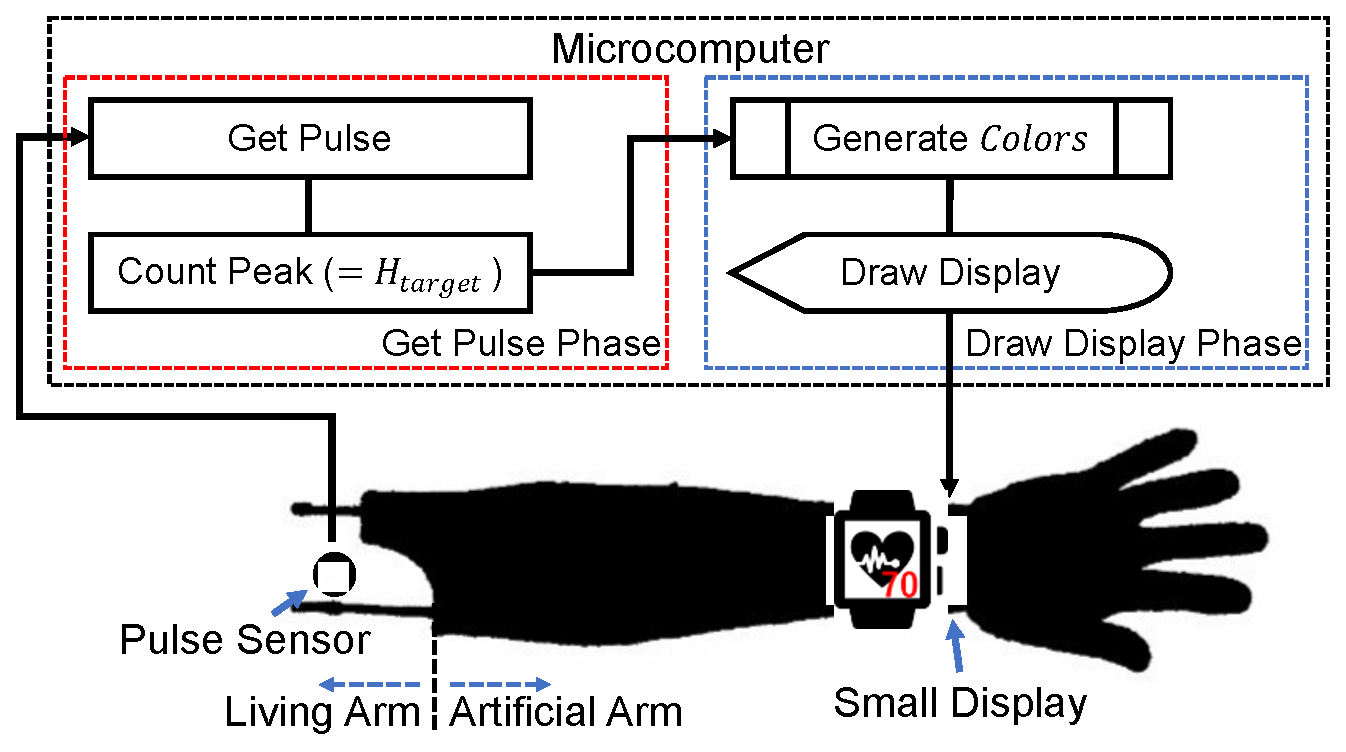
\includegraphics[width=0.75\linewidth]{figures/method.eps}
  \caption{Process flow of proposed method.}
  \label{fig:method}
\end{figure}


% 3.2
\subsection{Target Heart Rate Calculation}
The target heart rate that the proposed method lets the smartwatch measure is the wearer's heart rate obtained using another PPG sensor. Its value can be specified in real time. Let $H_{target}$ be the target heart rate. $H_{target}$ can also be given manually if the user wants the smartwatch to measure a specific heart rate.


% 3.3
\subsection{Display Control}
\label{subsec:display_control}
The brightness of the display is controlled so that the heart rate measured by the smartwatch becomes $H_{target}$. An array $Colors$ that holds the brightness of the display to let the smartwatch detect a single pulse is prepared in advance. The $Colors$ data is grayscale, a type of computer color representation that uses 256 levels (0--255) to represent shades of color from black to white. $Colors[i]~(i=0,\dots,L)$ whose length is $L$ is generated by the following equation.
\begin{equation}
  Colors[i]=\min\left(\sin\left(\frac{2\pi i}{L}\right)+1,1\right)*SCALE+BASE
\end{equation}
% \begin{enumerate}
%   \renewcommand{\labelenumi}{\arabic{enumi}.}
%   \item $Colors[i]=\sin\left(\frac{2\pi i}{L}\right)+1~(i=0,\dots,L)$
% %  \item $Colors[i]=Colors[i]+1$
%   \item $Colors[i]=1$ (if $Colors[i]>1$)
%   \item $Colors[i]=Colors[i]*SCALE+BASE$
% \end{enumerate}
We determined the values of $L$, $SCALE$, and $BASE$ heuristically in advance for each display-smartwatch combination. The PPG sensors irradiate infrared, red, or green LEDs onto the skin and measure the pulse data from the changes in light reflected through the blood vessels. Because blood flow increases with the timing of the pulse, more light is absorbed by the blood vessels, and the reflected light is dimmer. The smaller the grayscale, the closer it is to black. Since black absorbs more light than white, the more the display is rendered black, the darker the light emitted from the smartwatch worn on the display and reflected through the display.\par

The drawing interval $T=\frac{60}{L * H_{target}}$[s] for each value of $Colors$ is set so that $Colors$ is displayed $H_{target}$ times in one minute.
% \begin{equation}
%   \label{eqn:wait}
%   T = \frac{60}{L * H_{target}}
% \end{equation}
The proposed method draws the values of $Colors$ on the display $T$[s] one by one for each value.


% 3.4
\subsection{Pulse Data Measurement}
In the proposed method, a smartwatch is worn over a blinking display and pulse data is measured. Pulse data measured from a PPG sensor equipped on a smartwatch can be used in various applications. However, the performance of the PPG sensor and the algorithm for measuring the pulse data will vary depending on the model of the smartwatch, and are not disclosed to the public. For this reason, we set the target heart rate manually in our evaluation experiment. We then observe the error between the target heart rate and the heart rate measured by the smartwatch and investigate the effects of the smartwatch model and display.



% 4
\section{Evaluation}
\label{sec:evaluation}
This section describes the experiments we conducted to evaluate the effectiveness of the proposed method. We measured the heart rate acquired by a smartwatch when an arbitrary target heart rate was given.

% 4.1
\subsection{Display Control Software}
\label{subsec:software}
A program to change the brightness of the display was implemented using Python and Processing\footnote{\url{https://processing.org}}. First, Python receives the target heart rate $H_{target}$. Then, $T=\frac{60}{L * H_{target}}$[s] is calculated. Python sends $Colors[i]$ to Processing using its \texttt{socket} library and waits for the drawing to be completed. When Processing receives the data, it uses the \texttt{background} method to draw the grayscale as the background color of the window on the display. When the drawing is completed, Python receives a notification from Processing. If $T$[s] has passed, Python sends $Colors[i+1]$ to Processing. When all the data in $Colors$ has been sent, the $H_{target}$ is obtained and the system repeats this flow.


% 4.2
\subsection{Smartwatch Application}
\label{subsec:wearos}
A smartwatch is used to measure the heart rate. Smartwatches have different ways of acquiring heart rate depending on the operating system they have installed. In this subsection, we describe the methods of obtaining the heart rate for several OSs.


% 4.2.1
\subsubsection{Wear OS by Google}
TicWatch Pro WF12106 and PUMA Smartwatch were used in the evaluation experiment. These are both smartwatches run using Wear OS by Google\footnote{\url{https://wearos.google.com}}, which is an operating system designed for smartwatches based on Google's Android. We implemented the application using Android Studio\footnote{\url{https://developer.android.com/studio}}. The application stores heart rate data in the smartwatch storage in csv format. Sensor number 21 is used to acquire the heart rate data. The rate of events ``SENSOR\_DELAY\_UI'' is used to set a sampling rate suitable for the implementation of the user interface\footnote{\url{https://developer.android.com/reference/android/hardware/SensorManager}}.


% 4.2.2
\subsubsection{watchOS}
\label{subsec:applewatch}
Apple Watch Series 3 and Series 5 were used in the experiment. Apple Watch comes with a standard application that measures heart rate\footnote{\url{https://support.apple.com/en-us/HT204666}}. The collected heart rate data can be output as numerical data in XML format using the iPhone ``Health'' application paired with Apple Watch\footnote{\url{https://support.apple.com/guide/iphone/share-health-and-fitness-data-iph27f6325b2/ios}}.


% 4.2.3
\subsubsection{Original OS}
\label{subsec:original}
The SMART R F-18 used in the experiment is equipped with a proprietary operating system developed by the manufacturer. Heart rate data collected by this smartwatch can be viewed on the ``WearHealth'' application developed for Android and iPhone\footnote{\url{https://play.google.com/store/apps/details?id=com.zjw.wearhealth}}.


% 4.3
\subsection{Evaluation Environment}
TicWatch Pro WF12106, PUMA Smartwatch, Apple Watch Series 3 and Series 5, and SMART R F-18 were used for the evaluation experiment. For the display, we used the laptop display of Legion 7 15IMH05 by Lenovo (Display A), two small 3.5-inch displays designed for Raspberry Pi by ELECROW and OSOYOO (Displays B and C), and a lightweight flexible display \cite{flexible_display} (Display D) we made. The smartwatches and displays A, B, and C are shown in \figref{smartwatches}, and Display D is shown in \figref{flexible}. When using Display D, only SMART R was able to acquire the heart rate correctly, so only this smartwatch was used in the evaluation experiment of Display D.

\begin{figure}[!t]
  \centering
  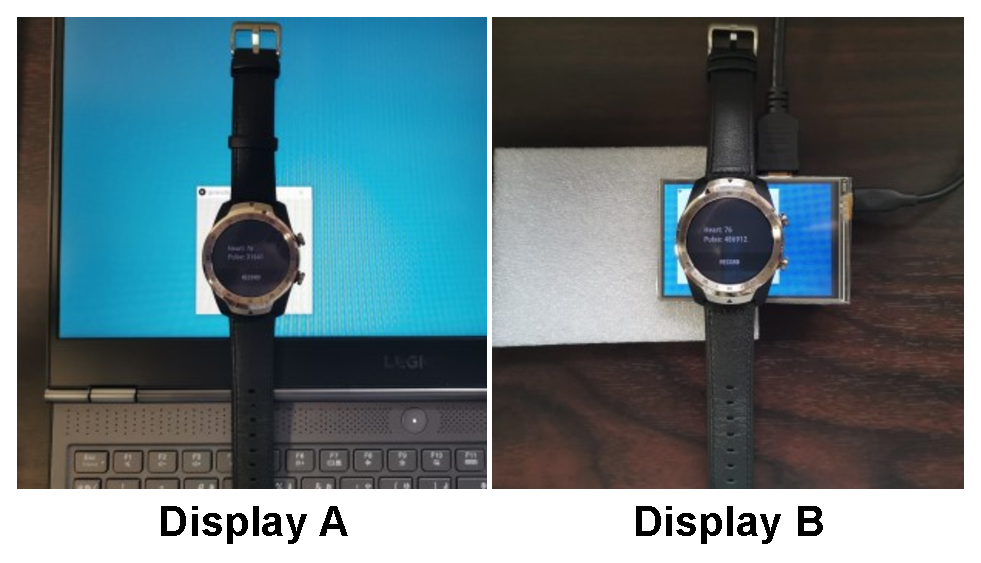
\includegraphics[width=0.78\linewidth]{figures/smartwatches.eps}
  \caption{Smartwatches and displays used in the experiment.}
  \label{fig:smartwatches}
\end{figure}

\begin{figure}[!t]
  \centering
  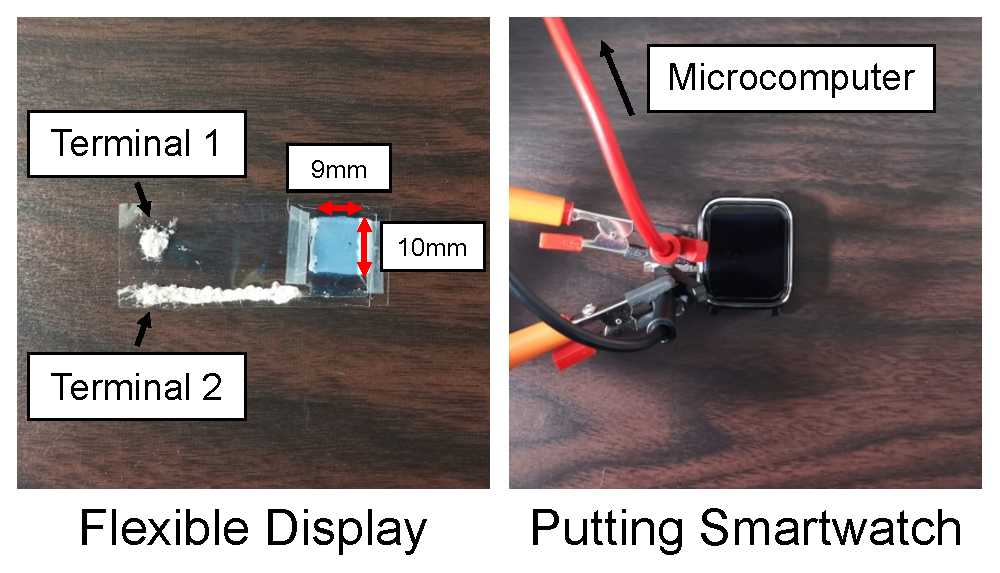
\includegraphics[width=0.75\linewidth]{figures/flexible.eps}
  \caption{Appearance of the flexible display (Display D).}
  \label{fig:flexible}
\end{figure}


\begin{table*}[!t]
\small
  \centering
  \caption{Error of heart rate obtained by TicWatch Pro, PUMA Smartwatch, Apple Watch Series 3, Apple Watch Series 5, and SMART R. (Display A: Lenovo Legion 7, B: 3.5-inch ELECROW, C: 3.5-inch OSOYOO, D: flexible display) }
  \begin{tabular}{c|ccc|ccc|ccc|ccc|cccc} 
  \toprule
    &\multicolumn{3}{c|}{TicWatch Pro}&\multicolumn{3}{c|}{PUMA}&\multicolumn{3}{c|}{Series 3}&\multicolumn{3}{c|}{Series 5}&\multicolumn{4}{c}{SMART R} \\
    $H_{target}$ & A & B & C & A & B & C & A & B & C & A & B & C & A & B & C & D \\
    \midrule
    $60$ & $-1.7$ & $-1.4$ & $-1.4$ & $-1.7$ & $-1.4$ & $-1.4$ & $0.4$ & $1.0$ & $-0.2$ & $58.2$ & $0.1$ & $-0.1$ & $-1.7$ & $-1.0$ & $-1.7$ & $-0.7$ \\
    $65$ & $-1.8$ & $-1.4$ & $-1.3$ & $-1.8$ & $-1.4$ & $-1.3$ & $0.6$ & $0.1$ & $-0.1$ & $16.1$ & $-0.4$ & $0.1$ & $-1.7$ & $-1.0$ & $-0.7$ & $-0.7$ \\
    $70$ & $-1.8$ & $-2.1$ & $-1.2$ & $-1.8$ & $-2.1$ & $-1.2$ & $0.1$ & $2.0$ & $0.0$ & $1.6$ & $2.4$ & $0.1$ & $-1.0$ & $-1.3$ & $-1.3$ & $-0.7$ \\
    $75$ & $-2.2$ & $-1.6$ & $-1.5$ & $-2.2$ & $-1.6$ & $-1.5$ & $0.0$ & $2.8$ & $-0.6$ & $0.8$ & $0.1$ & $-0.2$ & $-2.0$ & $-2.3$ & $-2.0$ & $-0.7$ \\
    $80$ & $-2.0$ & $-1.5$ & $-1.1$ & $-2.0$ & $-1.5$ & $-1.1$ & $-0.5$ & $1.0$ & $-0.5$ & $1.2$ & $0.9$ & $-0.4$ & $-2.0$ & $-2.0$ & $-1.0$ & $-1.0$ \\
    $85$ & $-1.8$ & $-1.5$ & $-1.6$ & $-1.8$ & $-1.5$ & $-1.6$ & $-5.4$ & $-0.7$ & $-0.6$ & $-0.6$ & $-1.0$ & $-0.9$ & $-2.0$ & $-2.0$ & $-1.7$ & $-0.7$ \\
    $90$ & $-2.0$ & $-1.7$ & $-1.0$ & $-2.0$ & $-1.7$ & $-1.0$ & $-0.6$ & $-1.3$ & $-0.6$ & $4.3$ & $-1.0$ & $-0.9$ & $-3.3$ & $-2.3$ & $-1.7$ & $-1.0$ \\
    $95$ & $-2.0$ & $-1.2$ & $-1.1$ & $-2.0$ & $-1.2$ & $-1.1$ & $-1.5$ & $-0.5$ & $-1.0$ & $-0.1$ & $-0.3$ & $-1.1$ & $-2.7$ & $-2.0$ & $-2.0$ & $-0.3$ \\
    $100$ & $-1.9$ & $-1.5$ & $-1.4$ & $-1.9$ & $-1.5$ & $-1.4$ & $-0.7$ & $-1.1$ & $-0.7$ & $-0.2$ & $-7.3$ & $-0.8$ & $-2.7$ & $-2.3$ & $-2.7$ & $-1.0$ \\
    \midrule
    Average & $-1.9$ & $-1.5$ & $-1.3$ & $-1.9$ & $-1.5$ & $-1.3$ & $-0.8$ & $0.4$ & $-0.5$ & $9.0$ & $-0.7$ & $-0.5$ & $-2.1$ & $-1.8$ & $-1.6$ & $-0.7$ \\
    \bottomrule
  \end{tabular}
  \label{tab:result}
\end{table*}

HDMI was used to connect Displays B and C to the laptop running the display control program. Display D is made of a flexible film that can fit on curved areas like the arm or the back of the Apple Watch, but it does not have HDMI. It blinks by switching the potential direction applied to the terminals. We implemented a system to run the proposed method described in Section \ref{sec:method} using the Arduino Uno R3 microcomputer. This microcomputer can control the output voltage by pulse width modulation (PWM). It receives the target heart rate from Python running on a computer connected to it and then changes the voltage to the display. The color of the display becomes darker when a higher voltage is applied to electrode 1 and lighter when a higher voltage is applied to electrode 2. The voltage of each electrode was switched between LOW and HIGH every $30/H_{target}$ seconds to let the smartwatch measure the target heart rate.\par

To obtain the correct heart rate, a 2-mm acrylic plate was placed between the display and a smartwatch in some display-smartwatch combinations. The smartwatches were placed on the display and the target heart rate was input to the display drawing program. The target heart rate was tested from 60 to 100 beats per minute (bpm) in increments of 5, which is a resting heart rate range for adults\footnote{\url{https://www.heart.org/en/healthy-living/fitness/fitness-basics/target-heart-rates}}. For the wearOS and watchOS smartwatches, heart rate was recorded for 60 seconds and the averaged measurement was used for the evaluation. For the originalOS smartwatch, heart rate was recorded once after 30 seconds due to limitations of the logging software. Heart rate measurement was conducted three times for each condition.


% 4.4
\subsection{Results and Discussion}
The error of the measured heart rate was calculated by subtracting the measurement from the target.
The results of the evaluation experiment are shown in \tabref{result}, where the results are the average of three sets.
% The results of the evaluation experiment using TicWatch Pro, PUMA Smartwatch, Apple Watch Series 3, Apple Watch Series 5, and SMART R are shown in \tabref{result}, where the results are the average of three sets.
Zero means that the heart rate was the same as the target heart rate, and minus means that the heart rate was smaller.
% The average errors for each display are also shown.


% 4.4.1
\subsubsection{WearOS Smartwatch}
The results showed that the heart rate could be input to the smartwatch within an error of less than $-3$ bpm. In both wearOS smartwatch results, the average error was smaller for Displays A, B, and C, in that order. This suggests that differences in performance, such as display brightness and refresh rate, may affect the generated heart rate.


% 4.4.2
\subsubsection{WatchOS Smartwatch}
The results showed that using Display C enabled the heart rate to be input to the Apple Watch within an error of $-1.1$ to $0.1$ bpm. On the other hand, when using Display A or B, it was not possible to obtain the correct heart rate under some conditions. In particular, when the target heart rate was set to 60 with the combination of Apple Watch Series 5 and Display A, the correct heart rate was not obtained even once.
% However, there were many cases where the heart rate was obtained correctly.


% 4.4.3
\subsubsection{Original OS Smartwatch}
The results showed that the heart rate could be input to the smartwatch within an error of almost less than $-3$ bpm. Especially for Display D, the heart rate could be input to the smartwatch within an error of less than $-1$ bpm.



% 5
\section{Conclusion}
\label{sec:conclusion}
In this paper, we proposed a method that enables a PPG sensor to measure an arbitrary heart rate using a display. We implemented a display drawing program and conducted an evaluation experiment using five kinds of smartwatches and four kinds of displays to determine the effectiveness of the proposed method. The results showed that the error between the target heart rate and the heart rate acquired by the smartwatch was within $\pm{3}$ beats per minute in many cases.
In future work, we will %improve the reproducibility of PPG data for use in a real environment and 
implement a mechanism that enables the wearable device worn on the display to measure the same PPG data by inputting PPG data obtained from a live body part. To achieve this, the system needs to automatically determine the colors to be drawn on the display, so we will build a generative model that can output the color to be drawn by inputting PPG data. We will also evaluate the effectiveness of the proposed method with a heart rate measured during sleep and exercise (40--180 bpm).


\begin{acks}
 Part of this work was supported by the Japan Science and Technology Agency PRESTO (JPMJPR1937) (JPMJPR20B7), The Takano Science Foundation, Yazaki Memorial Foundation for Science and Technology, and Tateishi Science and Technology Foundation. We thank Dr. Shuhei Tsuchida at Kobe University for connecting us to this collaborative research.
\end{acks}


% \section{Acknowledgments}

% Identification of funding sources and other support, and thanks to
% individuals and groups that assisted in the research and the
% preparation of the work should be included in an acknowledgment
% section, which is placed just before the reference section in your
% document.

% This section has a special environment:
% \begin{verbatim}
%   \begin{acks}
%   ...
%   \end{acks}
% \end{verbatim}
% so that the information contained therein can be more easily collected
% during the article metadata extraction phase, and to ensure
% consistency in the spelling of the section heading.

% Authors should not prepare this section as a numbered or unnumbered {\verb|\section|}; please use the ``{\verb|acks|}'' environment.

% \section{Appendices}

% If your work needs an appendix, add it before the
% ``\verb|\end{document}|'' command at the conclusion of your source
% document.

% Start the appendix with the ``\verb|appendix|'' command:
% \begin{verbatim}
%   \appendix
% \end{verbatim}
% and note that in the appendix, sections are lettered, not
% numbered. This document has two appendices, demonstrating the section
% and subsection identification method.

% \section{SIGCHI Extended Abstracts}

% The ``\verb|sigchi-a|'' template style (available only in \LaTeX\ and
% not in Word) produces a landscape-orientation formatted article, with
% a wide left margin. Three environments are available for use with the
% ``\verb|sigchi-a|'' template style, and produce formatted output in
% the margin:
% \begin{itemize}
% \item {\verb|sidebar|}:  Place formatted text in the margin.
% \item {\verb|marginfigure|}: Place a figure in the margin.
% \item {\verb|margintable|}: Place a table in the margin.
% \end{itemize}

%%
%% The acknowledgments section is defined using the "acks" environment
%% (and NOT an unnumbered section). This ensures the proper
%% identification of the section in the article metadata, and the
%% consistent spelling of the heading.
% \begin{acks}
% To Robert, for the bagels and explaining CMYK and color spaces.
% \end{acks}

%%
%% The next two lines define the bibliography style to be used, and
%% the bibliography file.
\bibliographystyle{ACM-Reference-Format}
\bibliography{references}

%%
%% If your work has an appendix, this is the place to put it.
% \appendix

% \section{Research Methods}

% \subsection{Part One}

% Lorem ipsum dolor sit amet, consectetur adipiscing elit. Morbi
% malesuada, quam in pulvinar varius, metus nunc fermentum urna, id
% sollicitudin purus odio sit amet enim. Aliquam ullamcorper eu ipsum
% vel mollis. Curabitur quis dictum nisl. Phasellus vel semper risus, et
% lacinia dolor. Integer ultricies commodo sem nec semper.

% \subsection{Part Two}

% Etiam commodo feugiat nisl pulvinar pellentesque. Etiam auctor sodales
% ligula, non varius nibh pulvinar semper. Suspendisse nec lectus non
% ipsum convallis congue hendrerit vitae sapien. Donec at laoreet
% eros. Vivamus non purus placerat, scelerisque diam eu, cursus
% ante. Etiam aliquam tortor auctor efficitur mattis.

% \section{Online Resources}

% Nam id fermentum dui. Suspendisse sagittis tortor a nulla mollis, in
% pulvinar ex pretium. Sed interdum orci quis metus euismod, et sagittis
% enim maximus. Vestibulum gravida massa ut felis suscipit
% congue. Quisque mattis elit a risus ultrices commodo venenatis eget
% dui. Etiam sagittis eleifend elementum.

% Nam interdum magna at lectus dignissim, ac dignissim lorem
% rhoncus. Maecenas eu arcu ac neque placerat aliquam. Nunc pulvinar
% massa et mattis lacinia.

\end{document}
\endinput
%%
%% End of file `sample-authordraft.tex'.
